
\documentclass[12pt]{article}

\usepackage[utf8]{inputenc}
\usepackage[bulgarian]{babel}
\usepackage{graphicx}
\usepackage{sidecap}  %required for side captions
\usepackage{amssymb}
\usepackage{amsmath}
\usepackage{hyperref}
\usepackage{commath}  
\usepackage{tcolorbox}
\usepackage[top=1.3in, bottom=1.5in, left=1.3in, right=1.3in]{geometry}


\begin{document}
	\begin{center}
        \LARGE{\textbf{Тема: Определяне на Sentiment на разговор}}
        
        \bigskip
        \Large{Предмет: Приложно-програмни интерфейси за работа с облачни архитектури с Амазон Уеб Услуги (AWS)}
        
        \medskip
        \Large{Изготвил: Антони Петев Добренов,фн: 81454, имейл: antoni.dobrenov@gmail.com}
        
        \medskip
        \Large{Лектор: доц. д-р Милен Петров, година: 2020}
        
        \bigskip
	\end{center}
    
    
  %  \newpage
    \tableofcontents
    \bigskip
    \bigskip
    \newpage
  
\section{Условие} 


\medskip

\noindent Качване на .mp3 файл на който е записан разговор - диалог, монолог. Този файл се анализира и се определя sentiment-a на разговора, той може да бъде позитивен, негативен, неутрален и миксиран.

\section{Въведение}

Този serverless application, представлява набор от няколко навързани AWS услуги. AWS S3 служи за съдържане на качените разговори под .mp3 формат, имаме AWS Lambda която използва качените файлове като ги анализира и ги предава на AWS Transcribe, което служи да направо JSON обект с информация за този mp3 file и също така служи за това да определи sentiment-a на разговора, след което информацията се записва в DynamoDB и експортвам API Gateway на endpoint, като можем да извличаме данни за разговори по техния sentiment.

\section{Теория}

AWS е огромна платформа, която може да послужи за направянето на всичко. Не случайно много голяма част от най-използваните приложения и сайтове са базирани на техните услуги. С използването на SAM и AWS Lambda, много лесно се вдига уеб приложение.

\section{Използвани технологии}
\begin{itemize}
    \item \textbf{AWS Lambda}
    \item \textbf{AWS S3}
    \item \textbf{AWS DynamoDB}
    \item \textbf{AWS CloudWatch} 
    \item \textbf{AWS API Gateway}
    \item \textbf{AWS SAM}
    \item \textbf{AWS Transcribe}

\end{itemize}

%\newpage

\section{Инсталация и настройки}
\noindent\textbf{Стъпка 1.} Правите git clone на репоситорито.

\medskip

\noindent\textbf{Стъпка 2.} Ако нямате aws-sam-cli, си го инсталирате : 
\begin{itemize}

\item  \noindent\textbf{Windows} - \url{https://docs.aws.amazon.com/serverless-application-model/latest/developerguide/serverless-sam-cli-install-windows.html}.

\item  \noindent\textbf{Linux} - \url{https://docs.aws.amazon.com/serverless-application-model/latest/developerguide/serverless-sam-cli-install-linux.html}. 

\item \noindent\textbf{MacOS} - \url{https://docs.aws.amazon.com/serverless-application-model/latest/developerguide/serverless-sam-cli-install-mac.html}.

\end{itemize}

\medskip

\noindent\textbf{Стъпка 3.} Кофигурирайте AWS креденшълите си - \url{https://docs.aws.amazon.com/serverless-application-model/latest/developerguide/serverless-getting-started-set-up-credentials.html}/

\medskip

\noindent\textbf{Стъпка 4.} Изпълнете \textcolor{blue}{sam deploy --guided} и завършете deploy-ването в AWS.

\medskip

\section{Кратко ръководство за потребителя}

\begin{itemize}

\item Записвате гласово съобщение под .mp3 форма.

\item Влизате в AWS Console, след което влизате в S3.

\item Избирате създадения от вас bucket.

  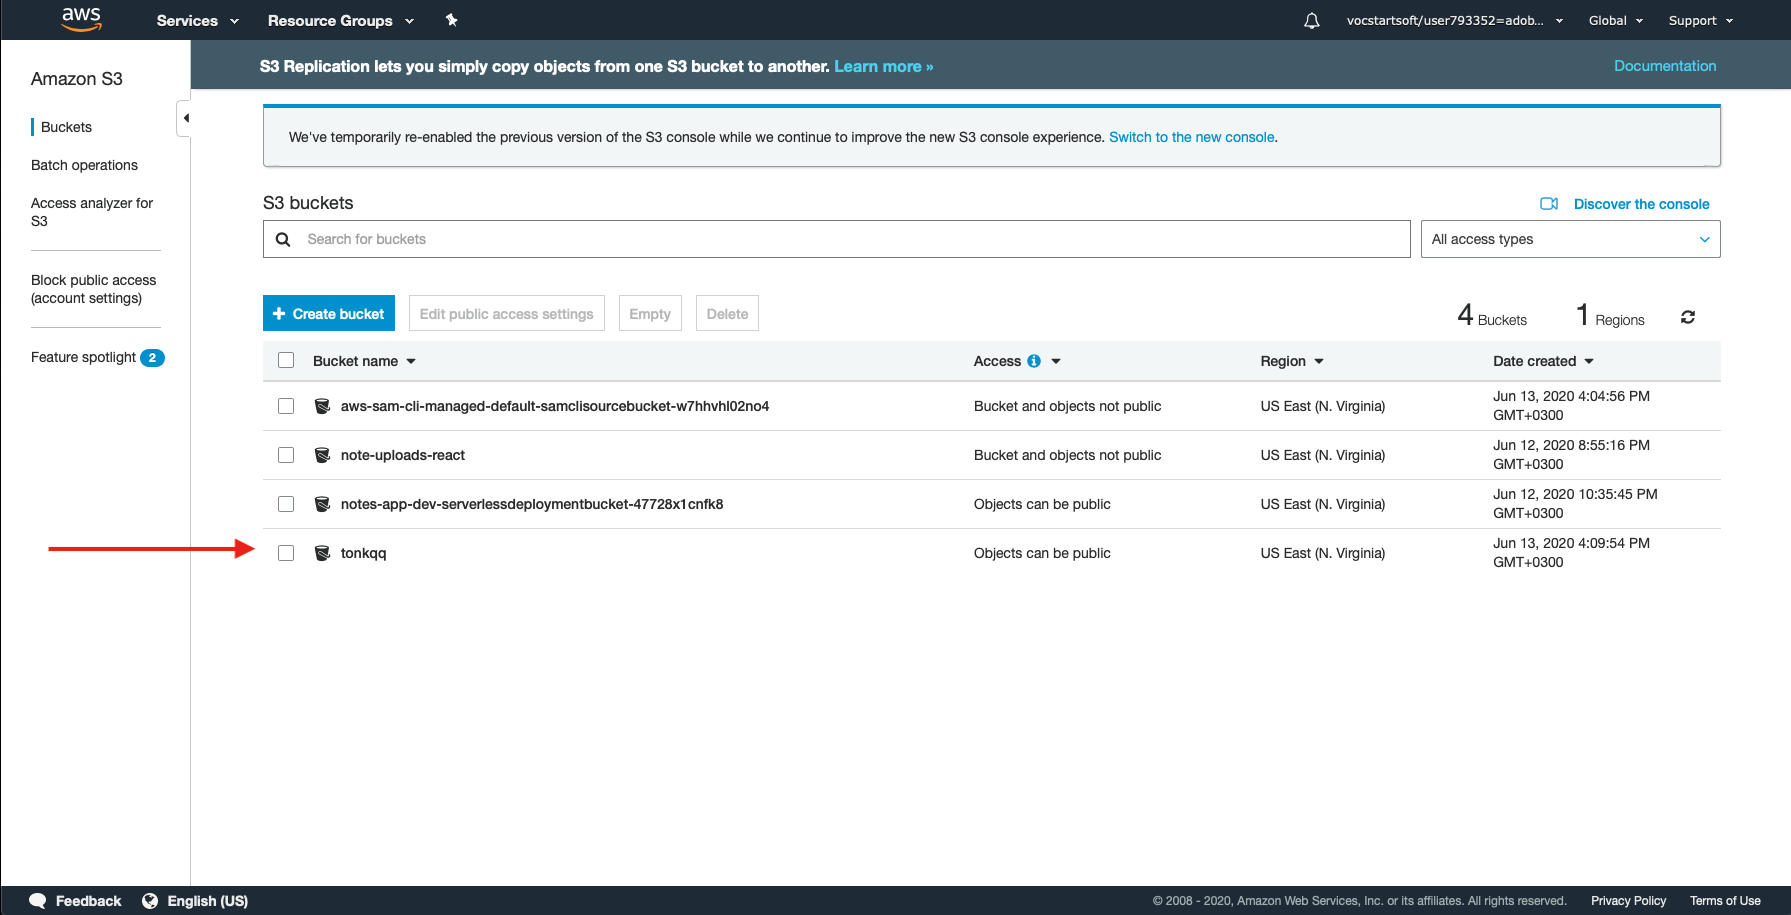
\includegraphics[width=0.8\textwidth]{choose_s3_bucket.png}

\item Настискате Upload и качвате файла/файловете.

 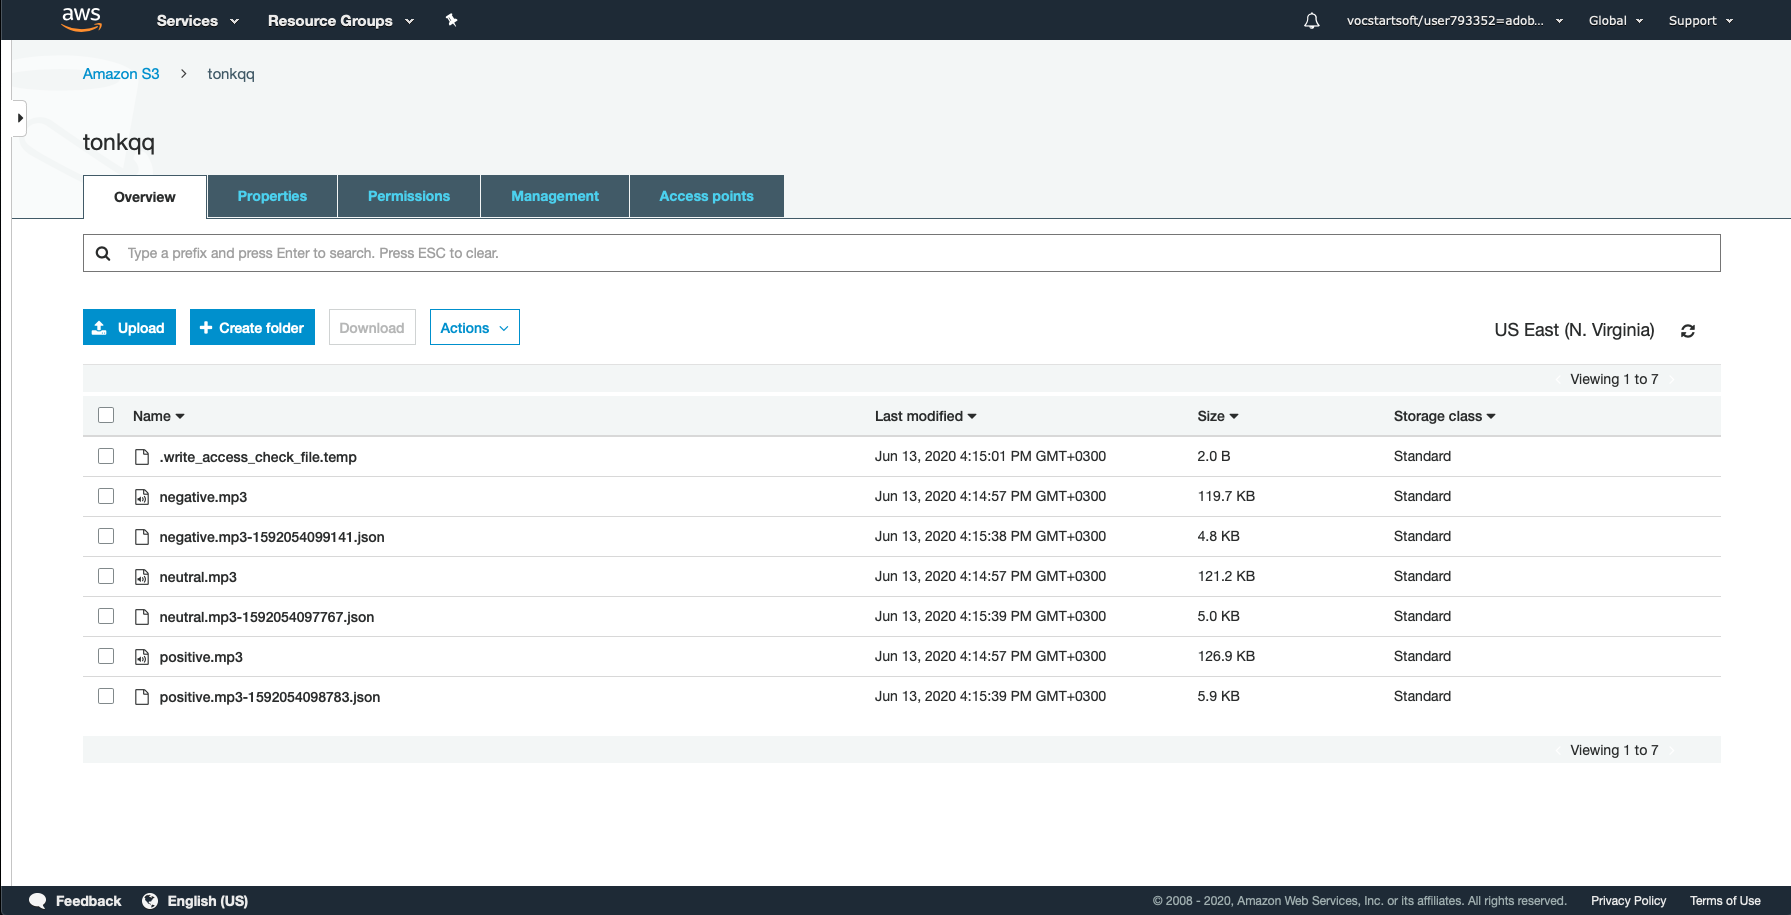
\includegraphics[width=0.8\textwidth]{upload_files.png}

\item Може да влезнете в DynamoDB и да видите информацията относно качените файлове.

 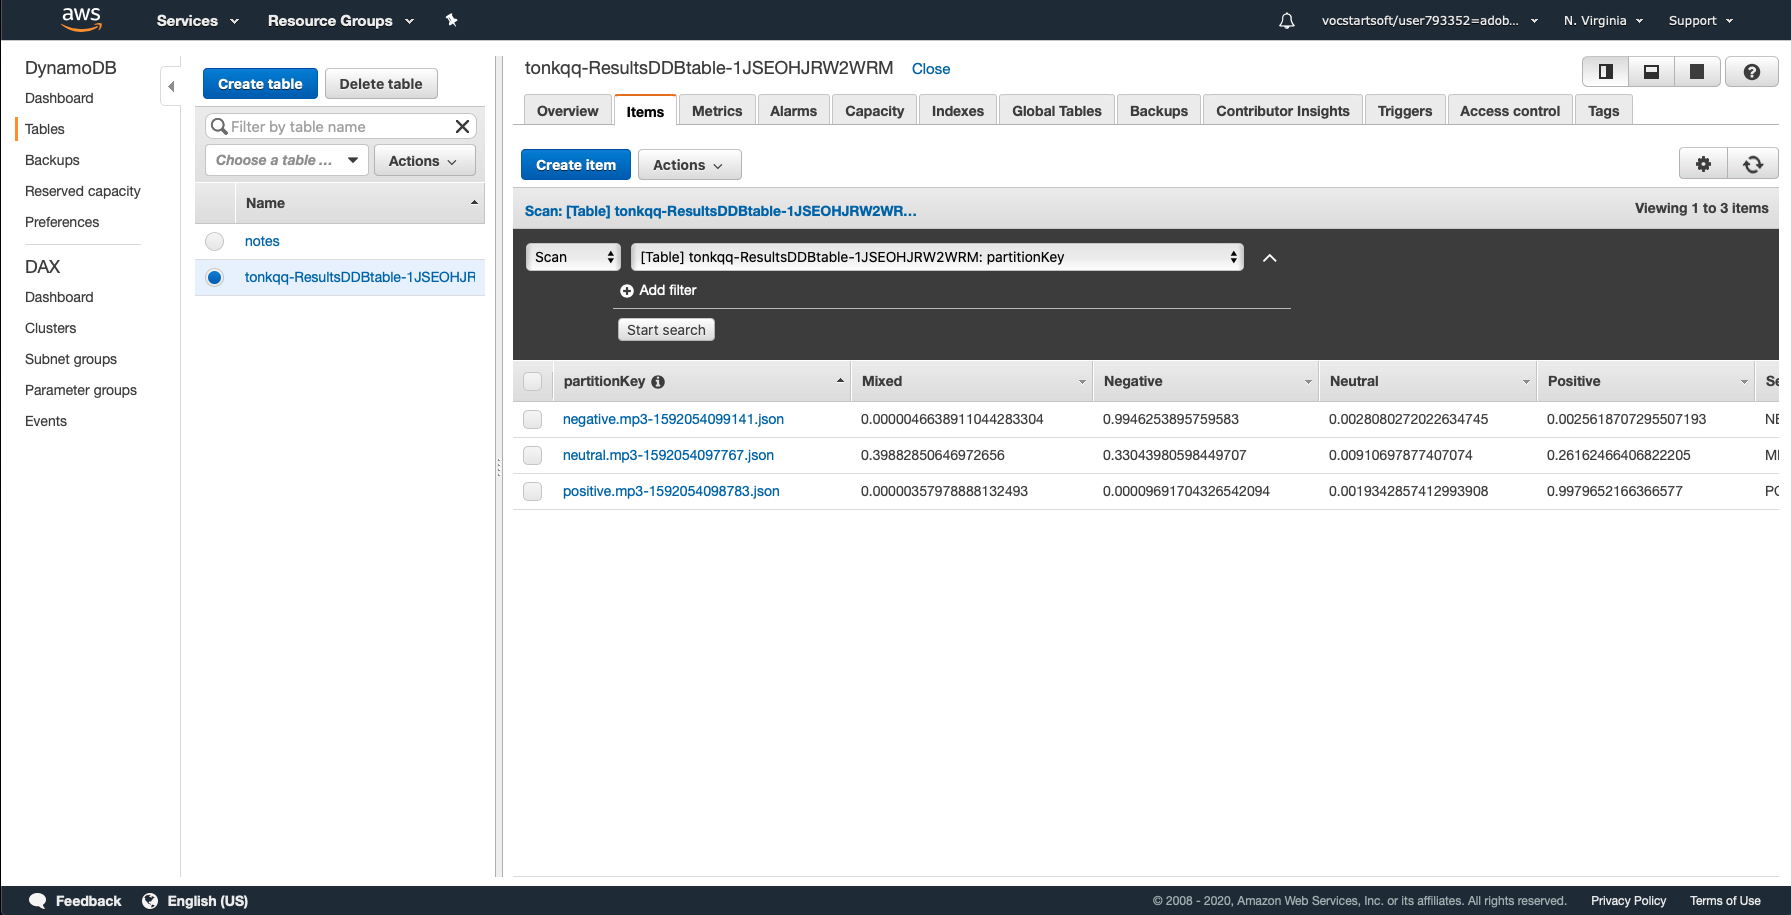
\includegraphics[width=0.8\textwidth]{check_dynamodb.png}

\item Може да влезете в API Gateway и да извикате endpoint-a като му зададете pathParameter - sentiment.

 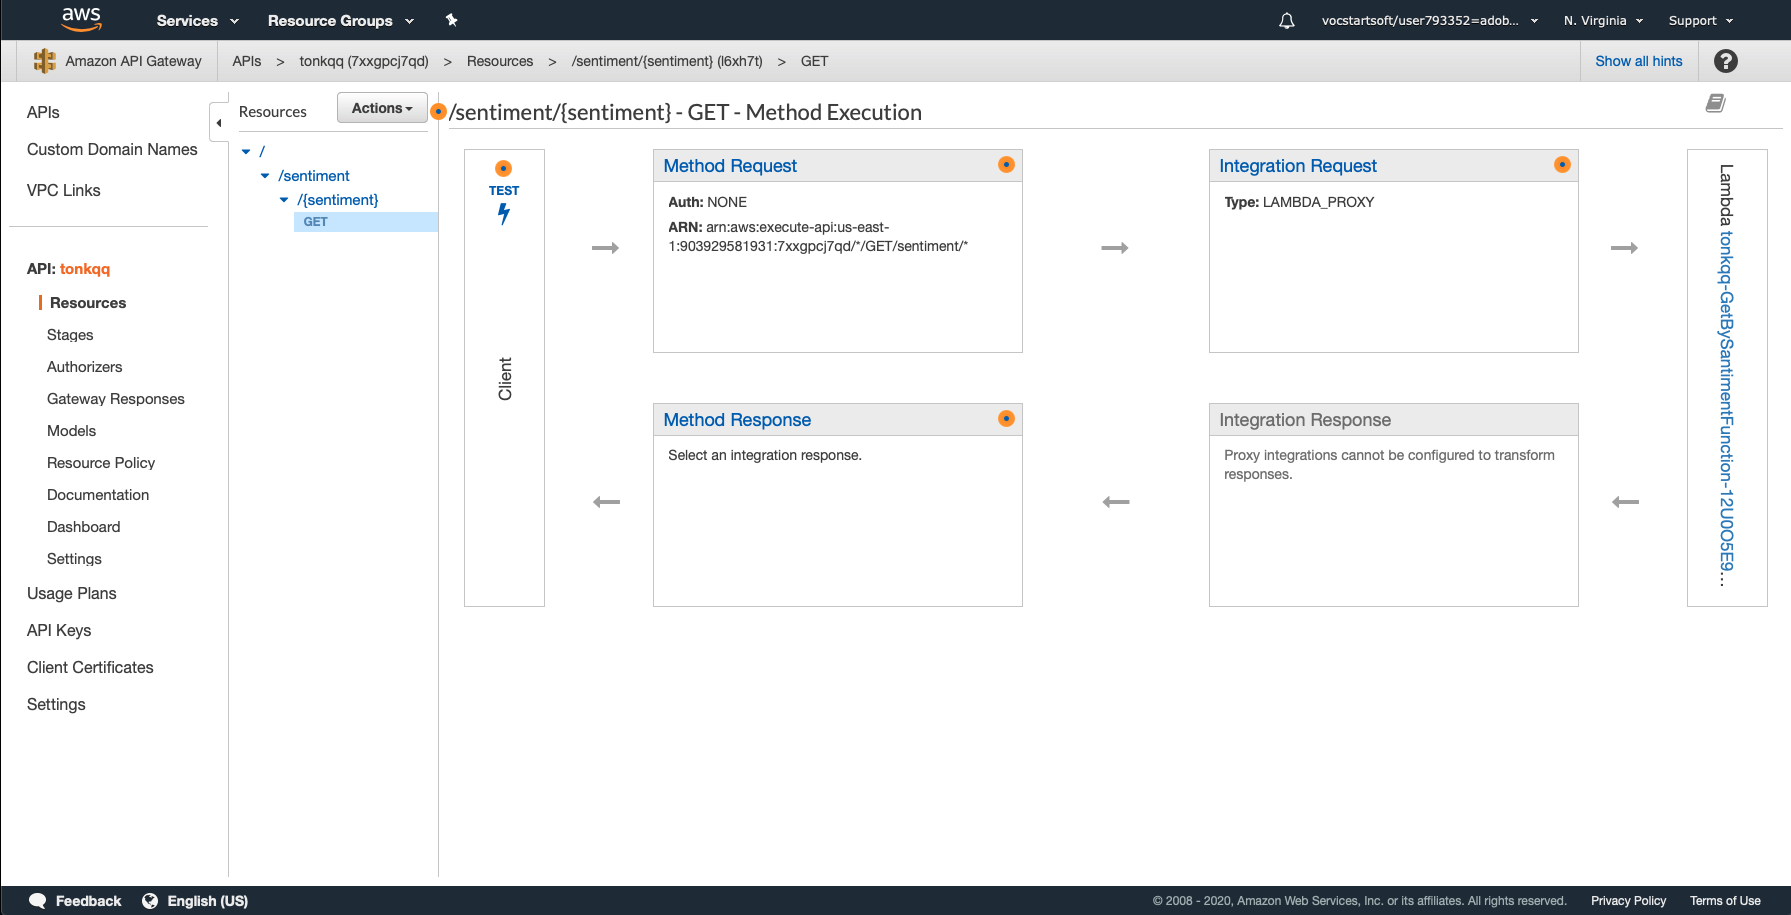
\includegraphics[width=0.8\textwidth]{check_api_gateway.png}
 
\item Преди да извикате endpoint-a например през Postman, трябва да се authenticate-нете: 

 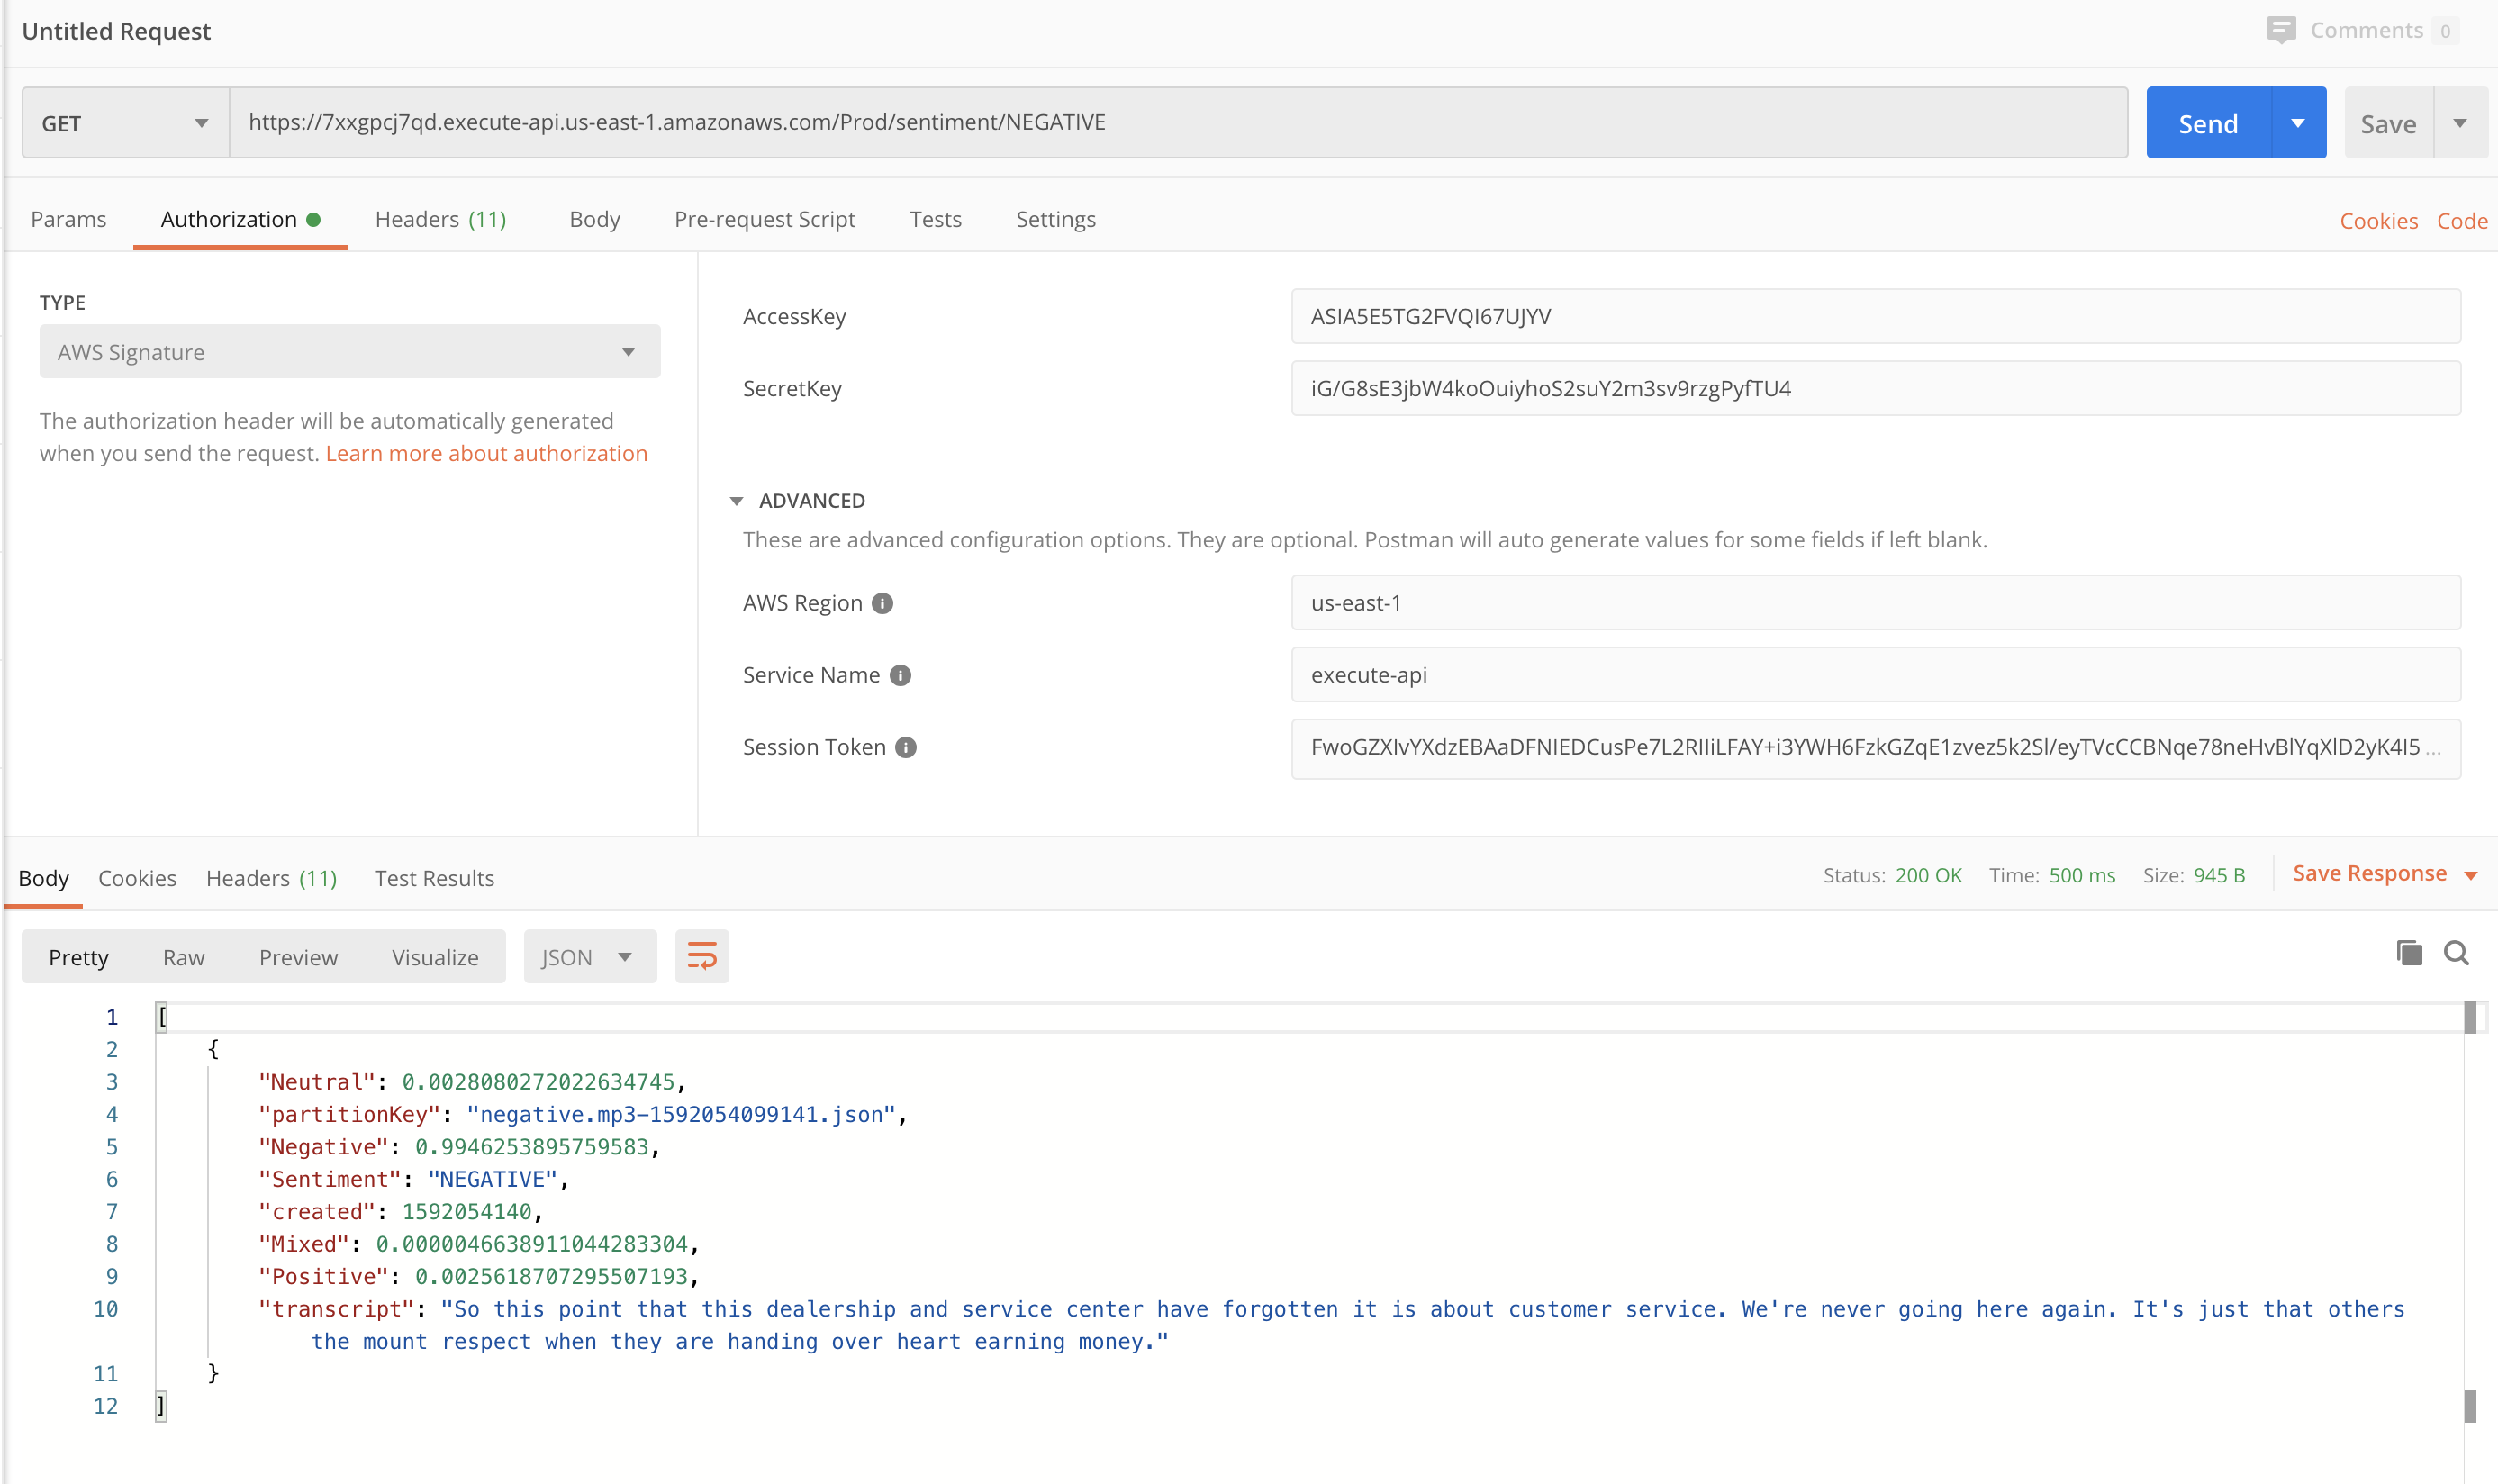
\includegraphics[width=0.8\textwidth]{postman_authenticate.png}
 
\end{itemize}

\section{Примерни данни}

Какъвто и mp3 file да качите в S3, след като влезнете в AWS Transcribe, той ще бъда показан там и ще можете да видите неговия json output.

\textcolor{blue}{
  "jobName": "negative.mp3-1592047622350",
  "accountId": "903929581931",
  "results": {
    "transcripts": [
      {
        "transcript": "So this point that this dealership and service center have forgotten it is about customer service. We're never going here again. It's just that others the mount respect when they are handing over heart earning money."
      }
    ],
    "items": [
      {
        "start_time": "0.74",
        "end_time": "1.15",
        "alternatives": [{ "confidence": "1.0", "content": "So" }],
        "type": "pronunciation"
      },
      {
        "start_time": "1.15",
        "end_time": "1.37",
        "alternatives": [{ "confidence": "1.0", "content": "this" }],
        "type": "pronunciation"
      },
      .....
      ]}}

Резултат от Postman

 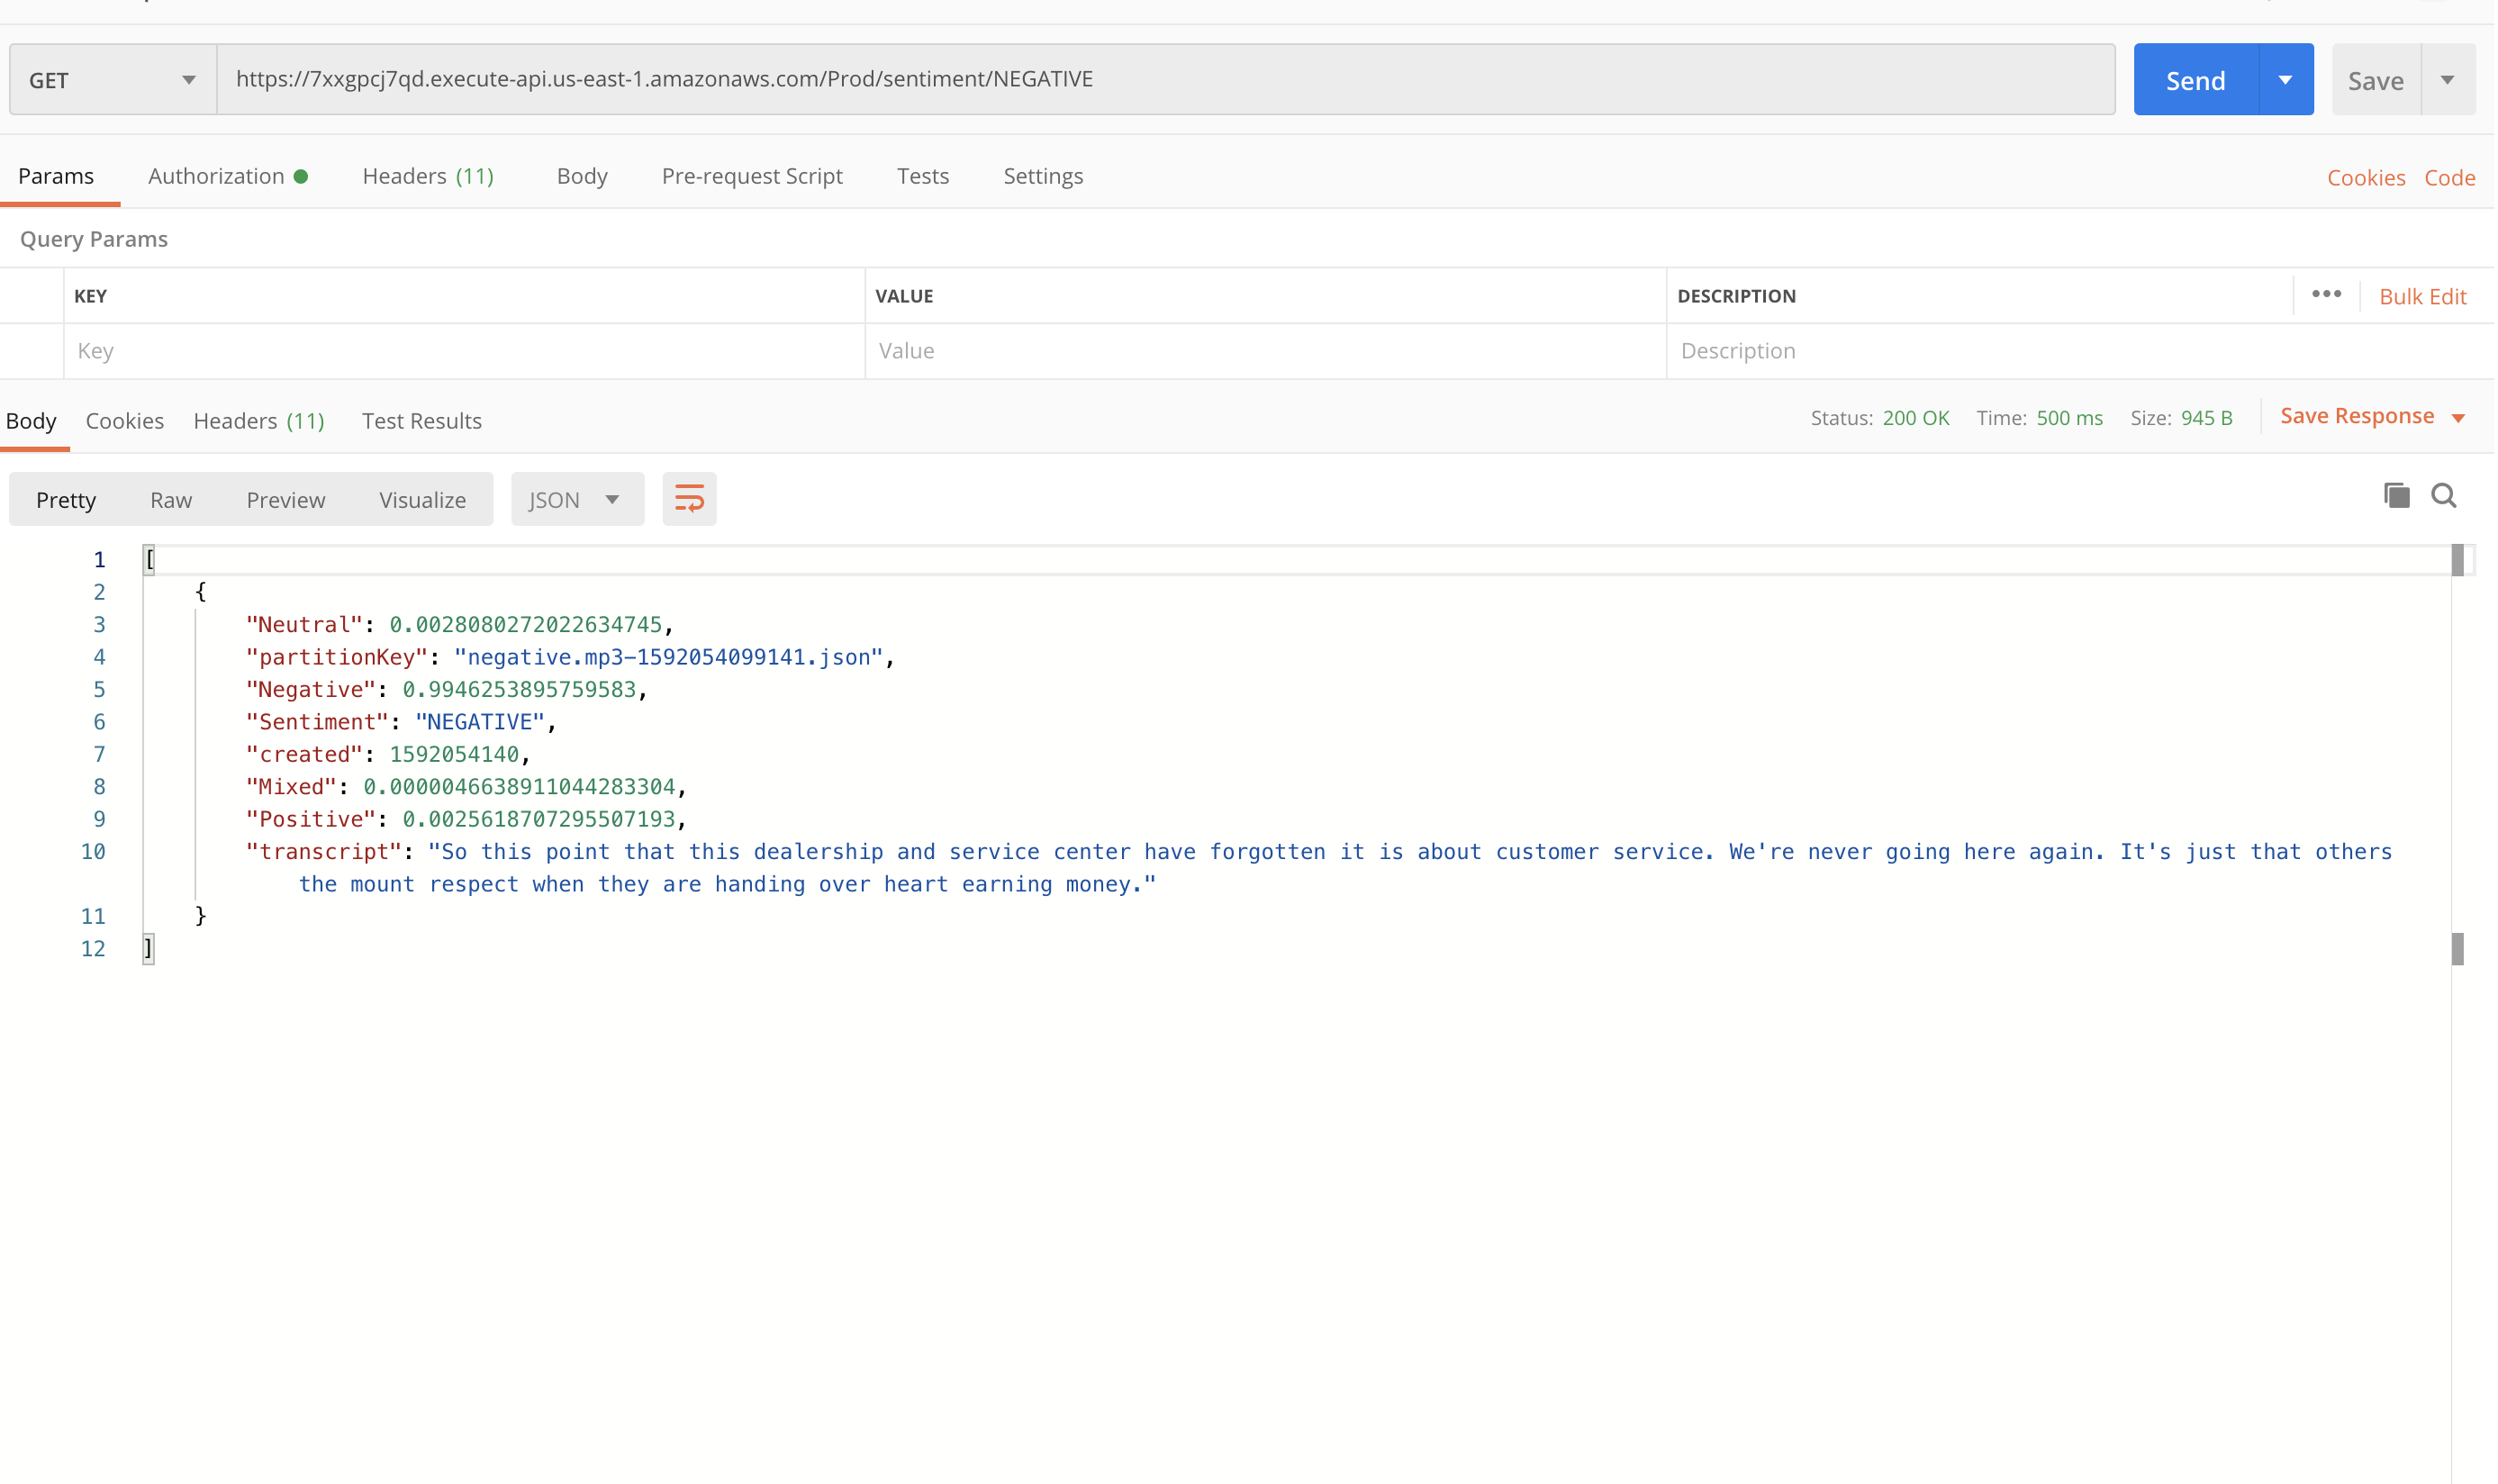
\includegraphics[width=0.8\textwidth]{postman_result.png}
 
\section{Описание на програмния код}

Състои се от 3 ламбда функции и template.yaml който служи за deploy на функциите.

\subsection{TranscribeFunction}
 Служи за извличане на файла от S3 и да извика startTranscriptionJob ot Transcribe service-a, което изслушва файла и създава горепосочения JSON обект.

\subsection{SentimentFunction}
Служи за обработване на този JSON обект и записването на данните от него в DynamoDB.

\subsection{GetSentimentFunction}
Служи за експортване на API Gateway, и при извикването на endpoint-a, претърсва DynamoDB за записите с подадения като параметър sentiment

\subsection{template.yaml}
В него се описват конфигурациите за deploy-ването на фунцкиите, създаването на DynamoDB Table, създаване на S3 bucket и определянето на ролите на функциите.

\medskip


\section{Приноси на студента, ограничения и възможности за бъдещо развитие}

Възможности за бъдещо развитие биха били следните неща - възможност за качване на mp3 file през API Gateway-a и интегриране с AWS SES, което би служило за изпращане на мейл, например когато се качи файл който е с негативен sentiment.

\medskip

\section{Какво научих}

Създаването на приложения с AWS е приятно и не толкова сложно, защото всеки service е направен така че да работи безпроблемно с който и да било друг service. Научих много за тези service-и които съм ползвал и също за други покрай тях.

\section{Списък с фигури и таблици}

\listoftables

\listoffigures

\section{Използвани източници}

\noindent\href{https://docs.aws.amazon.com/codedeploy/latest/userguide/tutorial-lambda-sam-template.html}{create sam}

\noindent\href{https://docs.aws.amazon.com/lambda/latest/dg/getting-started.html}{create lambda functions}

 \noindent\href{https://docs.aws.amazon.com/lambda/latest/dg/with-s3-example-use-app-spec.html}{integrate sam with s3}
 
 \noindent\href{https://docs.aws.amazon.com/serverless-application-model/latest/developerguide/serverless-getting-started-hello-world.html}{deploy sam}
\medskip

\bigskip

\end{document}
